\chapter{The nature of technical computing}
\label{chap:2}

The original numerical computing language was Fortran, short for
``Formula Translating System'', released in 1957.
Since those early days, scientists have dreamed of writing high-level,
generic formulas and having them translated automatically into low-level,
efficient machine code, tailored to the particular data types they
need to apply the formulas to.
Fortran made historic strides towards realization of this dream, and its
dominance in so many areas of high-performance computing is a testament to
its remarkable success.

The landscape of computing has changed dramatically over the years.
Modern scientific computing environments such as MATLAB~\cite{matlab},
R~\cite{Rlang}, Mathematica~\cite{mathematica}, Octave~\cite{Octave},
Python (with NumPy)~\cite{numpy}, and SciLab~\cite{scilab} have grown in popularity
and fall under the general category known as { {\it dynamic languages} or
{\it dynamically typed languages}.
In these languages, programmers write simple, high-level code without
any mention of types like \code{int}, \code{float} or \code{double} that
pervade statically typed languages such as C and Fortran.


%How should a computer scientist approach this space?
%We might try to maximize performance.

% so what should a future TC lang be?
% we cant just immitate and maximize the properties of existing
% systems.
% we have to look at the entire problem, and ask what can be
% fundamentally changed.

% these systems have many incidental features that have been
% criticized, but you can't solve the problem just by
% going through the design and fixing a few mistakes.
% once a system is basically the right thing, users will
% overlook flaws.


%Unfortunately,  is all to easy to make unfounded assumptions about
%what users want. But instead we should study the real world, see
%what is happening and figure out how to steer it in a better direction.

%Hypothesis: people don't know what they want. It's also hard to
%predict what people will want in the future. We need, in the words
%of Gerry Sussman, systems adaptable to uses not imagined by their
%designers.

\section{What is a technical computing environment?}

This question has not really been answered.
In fact technical computing software has been designed haphazardly.
Each system has evolved as a pile of features taken without what we
consider a sufficiently critical argument.

%Views of this are strongly shaped by what systems happen to exist,
%and what people were exposed to as they learned to program.

Some languages provide a ``convenient'' experience that is
qualitatively different from ``inconvenient'' languages.
We believe this can be made somewhat precise.
A large part of ``convenience'' is the reduction of the amount you need to know
about any given piece of functionality in order to use it.
This leads languages to adopt various forms of loose coupling,
automation, and elision of software engineering distinctions that are
considered important in other languages.

These systems are function-oriented, typically providing a rather
large number of functions and a much smaller number of data types.
Type definitions and features for organizing large systems are
de-emphasized.
But functions are heavily emphasized, and the functions in these
systems have a particular
character one might describe as ``manifest'': you just call them,
interactively, and see what they do.
This notion includes the following features:

\vspace{-3ex}
\begin{singlespace}
\begin{itemize}
\item Performing fairly large tasks in one function
\item Minimal ``set up'' work to obtain suitable arguments
\item No surrounding declarations
\item Permissiveness in accepting many data types and attempting to
      automatically handle as many cases as possible
\item Providing multiple related algorithms or behaviors under a single name
\end{itemize}
\end{singlespace}

Language design choices affect the ability to provide this user experience
(though the first two items are also related to library design).
Informally, in order to provide the desired experience a language needs to be
able to assign a meaning to a brief and isolated piece of code such as
\texttt{sin(x)}.
This leads directly to making declarations and annotations optional,
eliding administrative tasks like memory management, and leaving
information implicit (for example the definition scopes and types of the
identifiers \texttt{sin} and \texttt{x}).
These characteristics are strongly associated with the Lisp tradition of
dynamically typed, garbage collected languages with interactive REPLs.

However, there are subtle cultural differences.
A case in point is the MATLAB \texttt{mldivide}, or backslash, operator
\cite{matlabman:mldivide}.
By writing only \texttt{A\textbackslash B}, the user can solve square,
over- or under-determined linear systems that are dense or sparse, for multiple
data types.
The arguments can even be scalars, in which case simple division is performed.
In short, a large amount of linear algebra software is accessed via a
single character!
This contrasts with the software engineering tradition, where clarifying programmer
intent would likely be considered more important. %(TODO cite if possible?)
Even the Lisp tradition, which originated most of the convenience features
enumerated above, has sought to separate functionality into small pieces.
For example Scheme provides separate functions \texttt{list-ref} and
\texttt{vector-ref} \cite{schemelang} for indexing lists and vectors.

% now we will look at an example to motivate design discussion

\subsection{Case study: Vandermonde matrices}

To get a sense of how current technical computing environments work,
it is helpful to look at a full implementation example.
NumPy~\cite{numpy} provides a function for generating Vandermonde matrices
which, despite its simplicity, demonstrates many of the essential language
characteristics this thesis addresses.
The user-level \texttt{vander} function is implemented in Python (here
lightly edited for presentation):

\begin{singlespace}
\begin{lstlisting}[language=python,style=ttcode]
def vander(x, N):
  x = asarray(x)
  if x.ndim != 1:
    raise ValueError("x must be a one-dimensional array or sequence.")

  v = empty((len(x), N), dtype=promote_types(x.dtype, int))

  if N > 0:
    v[:, 0] = 1
  if N > 1:
    v[:, 1:] = x[:, None]
    multiply.accumulate(v[:, 1:], out=v[:, 1:], axis=1)

  return v
\end{lstlisting}
\end{singlespace}

This code has many interesting features.
Its overall structure consists of normalizing and checking arguments,
allocating output, and then calling the lower-level kernel \texttt{multiply.accumulate}
(written in C) to run the inner loop.
Even though most of the work is done in C, notice why this part of the
code is written in Python.
\texttt{vander} accepts nearly anything as its first argument, relying on
\texttt{asarray} to convert it to an array.
There is no need to write down requirements on argument \texttt{x}, allowing
the set of supported inputs to grow easily over time.
Next, an output array of the correct size is allocated.
The key feature of this line of code is that the data type to use is
\emph{computed} using the function \texttt{promote\_types}.
This kind of behavior is difficult to achieve in statically-typed languages.

The call to \texttt{multiply.accumulate} invokes a C function called
\texttt{PyUFunc\_Accumulate}, which is over 300 lines long.
The job of this function is to look up an appropriate computational
kernel to use given the types of the input arguments and the operation
being performed (\texttt{multiply}).
In other words, it performs dynamic dispatch.
This is notable because Python itself is already based on dynamic dispatch.
However, Python's class-based dispatch system is not particularly helpful
in this case, since the code needs to dispatch on multiple values.
Therefore NumPy's C code implements a custom dispatch table.
The targets of this dispatch are many compact, specialized
loops generated by running C code through a custom preprocessor.

The mechanism is complicated, but the results are appealing:
NumPy code has full run-time flexibility, yet can still achieve
good inner-loop performance.
Notice that this result is obtained through a clever, if painstaking,
mixture of binding times.
Python performs some late-bound operations, then calls an early-bound
C routine, which performs its own late-bound dispatch to a loop of
early-bound operations.

A central message of this thesis is that this kind of program behavior
is useful, highly characteristic of technical computing,
and can be provided automatically at the language level.
Here is how the above dispatch scheme might be implemented in Julia
(mirroring the structure of the Python code as much as possible to
facilitate comparison):

\begin{singlespace}
\begin{lstlisting}[language=julia]
function vander(x, N::Int)
  x = convert(AbstractVector, x)
  M = length(x)
  v = Array(promote_type(eltype(x),Int), M, N)
  if N > 0
    v[:, 1] = 1
  end
  if N > 1
    for i = 2:N; v[:, i] = x; end
    accumulate(MulFun(), v, v)
  end
  return v
end

function accumulate(op, input, output)
  M, N = size(input)
  for i = 2:N
    for j = 1:M
      output[j,i] = op(input[j,i], input[j,i-1])
    end
  end
end
\end{lstlisting}
\end{singlespace}

\noindent
This code implements the entire \texttt{vander} computation
(with some details left out, for example it does not provide the
\texttt{axis} argument of \texttt{multiply.accumulate}).
The C component is replaced by a general type-based dispatch system that
handles specializing and then invoking an efficient implementation of
\texttt{accumulate} for each combination of argument types.

% This code does not mention much about types or dispatch.
% many behaviors are implicit. e.g. how does indexing work?
% it's dispatch and specialization all the way down.

Performance is shown in table~\ref{vanderperf}.
When repeating the computation many times for small matrix sizes, the
overhead of the two-language dispatch system in NumPy completely
swamps computation time.
In the Julia \texttt{vander}, the type of \texttt{v} is known to the
compiler, so it is able to generate a direct call to the correct
specialization of \texttt{accumulate}, and there is no dispatch
overhead.
For large data sizes dispatch overhead is amortized, and NumPy
is much faster.
It is not clear why Julia is significantly faster in this case;
it may be due to NumPy's more general algorithm that can
accumulate along any dimension.
In that sense the comparison is not totally fair.
However, the Julia code for \texttt{accumulate} is so compact
that it is reasonable to write manually when needed; a fully
general library function is not required.

\begin{table}[!t]
\begin{center}
\begin{tabular}{|l|r|r|r|r|}\hline
\textbf{Size} & \textbf{\# iter} & \textbf{NumPy} & \textbf{Julia} & \textbf{Julia with dispatch} \\
\hline \hline
$4\times 4$        & 250000 & 5.43 & 0.072 & 0.204 \\
\hline
$2000\times 2000$  & 1 & 0.420 & 0.037 & 0.037 \\
\hline
\end{tabular}
\end{center}
\caption[Performance of \texttt{vander}]{
\small{
Time in seconds to compute \texttt{vander}, $4\times 10^6$ total points
arranged in many small matrices or one large matrix.
}
}
\label{vanderperf}
\end{table}

In some cases our compiler would not be able to determine the
type of \texttt{v}.
We simulated this situation and repeated the benchmark.
Results are shown in the rightmost column of the table.
Dispatch overhead is now significant for small data sizes.
However, performance is still fairly good, since there is only
a single layer of dispatch.
The dynamic dispatch logic exists in only one place in our code,
where it can be extensively optimized.

%% How much of the past 30 years of handwritten Matlab internals can
%% be autogenerated with a compiler? (A lot)

% now we extrapolate some general trends from this example

\section{Why dynamic typing?}

Mathematical abstractions often frustrate our attempts to represent them
on a computer.
Mathematicians can move instinctively between
isomorphic objects such as scalars and 1-by-1 matrices, but most programming
languages would prefer to represent scalars and matrices quite differently.
%A system might be able to convert automatically from one to the other, but
%it cannot always know which one we \emph{meant}.
Specifying interfaces precisely seems more rigorous, and therefore possibly
of use in mathematics, but technical users have voted with their code
not to use languages that do this.
A perennial debate occurs, for example, around the exact relationship
between the notions of \emph{array}, \emph{matrix}, and \emph{tensor}.
Informal interfaces, e.g. as provided by ``duck typing'', are a viable
way to share code among disciplines with different interpretations of
key abstractions.
It is not too surprising that dynamic typing is popular in the
technical computing world.

\subsection{Mismatches with mathematical abstractions}

Programs in general, deal with values of widely varying disjoint types:
functions, numbers, lists, network sockets, etc.
Type systems are good at sorting out values of these different types.
However, in mathematical code most values are numbers or number-like.
Numerical properties (such as positive, negative, even, odd, greater
than one, etc.) are what matter, and these are highly dynamic.

The classic example is square root (\texttt{sqrt}), whose result is complex
for negative arguments.
Including a number's sign in its type is a possibility, but this quickly gets
out of hand.
When computing eigenvalues, for example, the key property is matrix
symmetry.
Linear algebra provides many more examples where algorithm and data type
changes arise from subtle properties. These will be discussed in more
detail in section~\ref{sec:linalg}.

We must immediately acknowledge that static type systems provide
mechanisms for dealing with ``dynamic'' variations like these.
However, these mechanisms require deciding which distinctions
will be made at the type level, and once the choice is made
we are restricted in how objects of different types can be used.
In the domain of linear algebra, for example, it would be useful
to have matrices that are considered different types for some
purposes (e.g. having different representations), but not others
(e.g. different types of matrices can be returned from the same
function).


%Debates about what abstractions mean -- AbstractMatrix
%we thought we knew what it meant, but what about something like
%SymTridiagonal? It can implement most of what a dense matrix
%has, but it can't obey every invariant.


%% multiple common features underlie mathematical objects of different
%% types (e.g. numbers, sets, matrices). in some cases it makes sense to
%% consider numbers and matrices as the same kind of thing, and in other
%% cases it doesn't matter. A given type system is likely not to have
%% anticipated the particular common features that matter to your program,
%% making it more difficult to express an idea. A concrete example is
%% the matlab fragment
%% if condition
%%   idx = ':'
%% else
%%   idx = 1
%% end
%% where we want to select either an entire dimension or the first position
%% alone. The ':' and 1 are both indexes in this context, though they would
%% be of disjoint types in most programming languages.


% \subsection{Operational reasoning}

%% people tend to think about programs operationally, i.e. what it *does* when
%% it runs. for example writing
%% if false
%%   code
%% end
%% the code does not "occur" and therefore does not need to be valid

%% there is less to learn. with static languages you have to learn what happens
%% at both compile time and run time, when only run time really matters.

%% there is a desire to parameterize as much as possible. functions
%% accept parameters, so function calling ought to be sufficient to express
%% any desired parameterization.


\subsection{I/O and data-oriented programming}

Inevitably there is a need to refer to a datatype at run time.
A good example is file I/O, where you might want to say ``read $n$ double precision
numbers from this file''.
In static languages the syntax and identifiers used to specify data types for
these purposes are usually different from those used to specify ordinary types.
A typical example is a constant like \texttt{MPI\_DOUBLE} \cite{snir1998mpi}, which
is used to indicate the data type of an MPI message.
Many libraries, especially those for tasks like interacting with databases and file
formats, have their own set of such tags.
Using more than one of these libraries together can result in lots of boilerplate
code to map between tag systems.

Polymorphic languages provide better interfaces in these cases.
For example, C++ overloading can be used to provide the correct tag automatically
based on the type of a function argument.
However, these techniques only work for statically-known types.
Code like that in the \texttt{vander} example that determines types using arbitrary
computation is excluded.
Dynamic typing provides a complete solution.
Indeed, I/O examples are often used to motivate dynamic typing \cite{Abadi:1991:DTS:103135.103138}.
With dynamic typing, a single set of names can be used to refer to all types
regardless of binding time, and the user may write whatever code is convenient
to handle classifying data moving in and out of a program.


%\subsection{Flat metadata hierarchy}

%static types are approximations of dynamic types, so languages with static
%types inevitably assign two types to a location (both a static type and a
%dynamic type) where one would do. in some languages, like C++, the desire
%for performance or ease of implementation leads the compiler to make some
%decisions based on static types. this is confusing. if type declarations
%can be omitted, as in a type-inferred language, the situation is even worse
%since the static type of a value might not be apparent.


%% \section{The software stack is too complex}

%% Collapsing abstraction layers

%% \begin{itemize}
%% \item for numerical debuggability in particular
%% \item no time spent worrying about binding time
%% \item you will build a dynamic dispatch layer anyway, so build it in
%% \end{itemize}

%% language performance psychology:
%% if your language doesn't directly support efficient machine data types,
%% users will rewrite their code in C in order to get them, and then be
%% happy with the result (though not with the process).


\section{Tradeoffs in current designs}

Current systems accept certain design tradeoffs to obtain flexibility.
% TODO MORE

\iffalse
%``Ducking'' the issue of typing is not really possible.

NumPy essentially adds an extra type system to Python (the
\texttt{dtype} class).
For a long time, there was no existing compiler that was aware of
this type system.
One was finally implemented \cite{oliphant2012numba}, but there are also
other Python extensions and JITs with their own incompatible
type systems.

% TODO: example of PyPy needing to implement core numpy functions
% one by one manually.

% TODO: mention R a lot in this section

% hard to work with types in language that deliberately tries to obscure
%them from the user.
Dictionaries for everything (python, js) is the wrong default.
Almost every
type somebody wants has a fixed number of fields with fixed types.

This phenomenon is increasingly noticed in other domains, particularly
JavaScript and web programming.
Modern JavaScript implementations are quite fast, but Google's Dart language
is based on the premise that we could have a web language that is even faster,
and offers more productivity as well.
How so? Because Dart's designers observed that JavaScript programmers in
practice often write code that could be defined using traditional OO classes,
but the language does not support them.

Python is often described as a good glue language.
This means it is effectively used as an interface standard, a kind of
extended C ABI that makes it easier for libraries to interoperate,
and easier for users to access those libraries.
Something as straightforward as providing a standard N-dimensional numeric
array class (NumPy), which does not exist at the level of C, goes a long way.

However, we wish to point out that in this picture, Python is not
doing as much work as it might first appear.
Python does not make it easier to implement the functionality inside NumPy,
or other ``under the hood'' scientific libraries.
In many cases it creates more work, through the need to write wrappers and
interfaces for native code.

%Merely being ``dynamic'' (e.g. Python) should not be considered
%the gold standard of flexibility.
Although these systems permit tricks that can solve otherwise difficult
programming problems, this is not always the kind of flexibility that is needed.
When faced with the need to describe many functions with elaborate
behavior and many cases, one does not primarily need permissiveness,
but rather powerful and descriptive organizing principles.
\fi

\subsection{Vectorization}

The attitude of vectorization proponents has been somewhat famously
summarized as ``Life is too short to spend writing for loops.'' \cite{1998matlab}
The vectorized style has the following touted benefits:

\begin{enumerate}
\item One may write \texttt{sin(x)} to compute the sine of
all elements of \texttt{x}, which is much more compact than writing a loop.
\item Most execution time can be spent inside an expertly-written library,
taking advantage of special hardware (e.g. SIMD units or stream processors
like GPUs) and parallelism implicitly.
\item The performance of the high-level language being used becomes less
relevant.
\item The compiler can optimize across whole-array operations, potentially
drastically rearranging computations in a way that would be difficult to do
by examining one scalar operation at a time.
\end{enumerate}

Under close inspection, this argument begins to break down.

An equivocation takes place between being \emph{able} to write a loop
as \texttt{sin(x)} and being \emph{required} to.
The former is all we really want, and it is possible in any language that
supports some form of function overloading.
There is no inherent reason that a high-performance language like C++ or
Fortran cannot also support more compact, high-level notation.

Studies reveal that many real-world applications written in vectorization
languages actually do not spend most of their time in libraries
\cite{evaluatingR}.
It is possible for an interpreter to be so slow that it cancels
the advantage of optimized kernels for a range of realistic data sizes.

The final reason, enabling advanced optimizations, is compelling.
However at a certain point a ``vectorization bottleneck'' can be reached,
where performance is limited by expressing computations in terms of
in-memory arrays.
Figure~\ref{fig:vecperf} compares the operation rate of three different
algorithms for evaluating the polynomial $x^2+x-1$ over double precision
vectors of varying size.
The solid line describes a naive algorithm, where each operation allocates
a new array and fills it with one intermediate result (a total of three
arrays are needed for the full evaluation).
The dotted line algorithm is similar in spirit, except the three operations
are ``fused'' into a single loop.
Only one pass is made over the data and one new array is allocated.
Naturally performance is much better in this case, and advanced array
programming environments like APL \cite{APL} and ZPL \cite{ZPL} implement
this optimization.

\begin{figure}[!t]
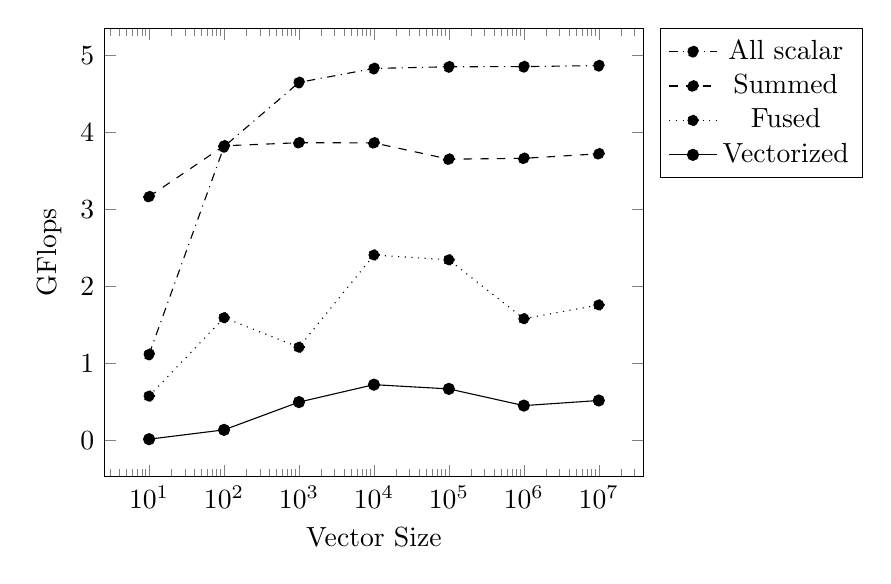
\begin{tikzpicture}
\begin{semilogxaxis}[
    %title=Vectorization Performance,
    xlabel={Vector Size},
    ylabel={GFlops},
    legend entries={Vectorized, Fused, Summed, All scalar},
    legend style={
      %at={(0.98,0.84)},
      legend pos = outer north east,
      anchor = north west,
      reverse legend=true
    },
]
\addplot+[color=black,mark=*,mark options={fill=black}] coordinates {
(10, 0.0181)
(100, 0.1390)
(1000, 0.5001)
(10000, 0.7263)
(100000, 0.6714)
(1000000, 0.4543)
(10000000, 0.5208)

};
\addplot+[color=black,mark=*,mark options={fill=black},style=dotted] coordinates {
(10, 0.5778)
(100, 1.5960)
(1000, 1.2126)
(10000, 2.4110)
(100000, 2.3484)
(1000000, 1.5835)
(10000000, 1.7621)

};
\addplot+[color=black,mark=*,mark options={fill=black},style=dashed] coordinates {
(10, 3.1693)
(100, 3.8297)
(1000, 3.8697)
(10000, 3.8677)
(100000, 3.6557)
(1000000, 3.6670)
(10000000, 3.7258)

};
\addplot+[color=black,mark=*,mark options={fill=black},style=dashdotted] coordinates {
(10, 1.1202)
(100, 3.8186)
(1000, 4.6531)
(10000, 4.8348)
(100000, 4.8566)
(1000000, 4.8585)
(10000000, 4.8718)

};
\end{semilogxaxis}
\end{tikzpicture}
\caption[Performance of vectorized code]{
\small{
  Performance of evaluating $x^2+x-1$ over a double precision vector of length $n$.
  Operation repeated $10^7/n$ times. (Core i7-3517U 1.9GHz, 4MB cache, 8GB RAM)
}
}
\label{fig:vecperf}
\end{figure}

However, this level of performance is not impressive compared to the
dashed line, which describes the operation rate for computing the
same results but summing them instead of storing them.
Finally, the dash-dotted line uses no memory at all, instead computing
input data points from a linear range.
Of course a real use case might require data to be read from memory or stored,
so this comparison is unfair (though not entirely, since many numerical
environments have represented even simple objects like linear ranges using
dense vectors \cite{matlabman:linspace}).
Still the point should be clear: vectors are not necessarily a good abstraction
for high performance.
The observation that memory is a bottleneck is not new, but for our purposes
the important point is that languages that only support vectorized syntax
cannot express the code rearrangements and alternate algorithms that can be
necessary to get the best performance.
A good technical computing language needs a more general interface to
performance.

The performance model resulting from vectorized syntax can be difficult to
understand, since it is difficult for users to predict which optimizations
will be applied.
A good example was discussed on the \texttt{julia-users} mailing list \cite{jasonmerrill}.
Jason Merrill discovered a Mathematica \cite{mathematica} list discussion
of the fastest way to count how many values fall within a given range.
Of many proposed implementations, the fastest turned out to be

\vspace{-3ex}

\[ \texttt{Total@Unitize@Clip[data,\{min,max\},\{0,0\}]} \]

\noindent
Arguably, it is difficult to know that this will run faster than, for
example,

\vspace{-3ex}

\[ \texttt{Count[data,~x\_/;~min<=x<=max]} \]

%% \begin{singlespace}
%% \begin{lstlisting}[language=julia]
%% function count_range(data, min, max)
%%     count = 0
%%     for elt in data
%%         if min < elt < max count += 1 end
%%     end
%%     count
%% end
%% \end{lstlisting}
%% \end{singlespace}

\iffalse
\subsection{What needs to be built in?}

It is often said that part of the usefulness of technical computing
environments comes from having many functions, and important abstractions
like matrices, ``built in''.

Built-in-ness often conflates two aspects:

\begin{enumerate}
\item A feature being readily available and agreed-on by all language users
\item A feature tightly coupled to the rest of the system
\end{enumerate}

(2) implies (1), but not the other way around. (2) is the only technically
interesting item, since the other can be addressed e.g.\  just by including
a library in the standard software distribution. Many technical computing
languages have done a large amount of (2) while justifying it with point (1).

While a large part of our motivation is to move more decisions and functionality
into libraries, it is equally important to identify what {\it must} be part of a
language for the system to be successful. We believe that large amounts of
functionality can be provided by add-ons, but that certain key features
cannot be. Past failures to properly classify features this way have
caused a lot of undue pain.

First, performance cannot be an add-on. If some users have a fast version of
a language and others have a slow version (with the difference being an
order of magnitude or more), library writers cannot be sure whether users
will find their code fast enough to be useful. How are we to teach people to
program in the language?

Psychologically, it may be difficult to accept a ``non standard'' extension
that changes a language so fundamentally. There is a nagging, though perhaps
totally unfounded, perception that something subtle may break. If indeed a
bug arises due to the use of such an extension, a user is likely to conclude
that the extension is dangerous or broken and stop using it. If, on the other
hand, a bug arises due to a language's standard optimizing compiler, the user
will simply file a bug report, then find a way to work around the problem.

Adding a JIT compiler to a language also requires acceptance of detriments
like compilation pauses and pages with RWX permissions. In some cases this
may lead to use of the extension being disallowed, perhaps for security
reasons.

Type systems similarly fail when provided as optional extensions. Library
writers face the same kinds of problems as with performance add-ons. Should I
use type annotations in my library?

Dynamic dispatch mechanisms also make especially poor add-ons. Of course,
every program makes decisions at run time, and so implements its own
``dispatch'' to some extent. But these behaviors are inextensible; if
language users do not agree on a reusable dispatch framework their code
will not be composable.
\fi

\subsection{Data representation}

There are two broad categories of programming language data models.
The first, favored by static languages, provides structures that are
complex and rigid but efficient.
Specific data types can be grouped and stored together with known
offsets and alignments.
Most data is stored directly, and pointer indirection must be
explicitly requested.
The second kind of data model, favored by dynamic languages,
prioritizes flexibility and simplicity.
Most data consists of pointers to tagged objects.
Indirection is the default.

It's reasonable to guess that these models would trade off about equally.
If you want the flexibility to substitute any kind of value in
any location at run time, making everything a pointer is the best
you can do.
The data layouts used by static languages require some
amount of metadata to describe, and manipulating this metadata
at run time could have significant overhead.
In the ``dynamic'' data model, even though everything is a pointer,
at least the code \emph{knows} that everything is a pointer, and so
does not waste time switching between different representations.

Interestingly, this intuition turns out not to be entirely true.
As memory performance becomes a larger bottleneck, using less
space and avoiding indirection becomes more important.
Furthermore, most data in dynamic language programs is not as
dynamic as its authors might think, with homogeneous arrays
being quite common.
Good evidence for this claim was documented as part of work on
\emph{storage strategies}~\cite{Bolz2013}, a technique for
adapting dynamic languages to use more efficient representations.
The authors found that it was worthwhile to represent an array
as a wrapper providing a heterogeneous array interface on top of
a homogeneous array of varying type, even at the expense of
extra dispatch and occasionally changing the representation.

% ``storage strategies'' is simultaneously a great idea, and also a crack
% in the armor of typical dynamic languages big enough to tear them apart.

In some sense, our work takes this idea to its logical conclusion:
why not support a range of data representations from the beginning,
managed by a single sufficiently powerful dispatch system?
% so you need some type system, might as well be a good one


\section{A compiler for every problem}

In several prominent cases the language of a scientific sub-discipline is
so far removed from conventional programming languages, and the need for
performance is so great, that practitioners decide to write their own
compilers.
For example, the Tensor Contraction Engine~\cite{baumgartner2005synthesis}
accepts a mathematical input syntax describing tensor operations
used for electronic structure calculations in quantum chemistry.
The software performs many custom optimizations and finally generates
efficient parallel Fortran code.
Other examples of such scientific code generators include
Firedrake~\cite{Rathgeber2015} and FEniCS~\cite{LoggOlgaardEtAl2012a}
for FEM problems, PyOP2~\cite{pyop2} for general computations on meshes,
FFTW~\cite{FFTW05} for signal processing, and Pochoir~\cite{tang2011pochoir}
for stencil computations.

%\begin{itemize}
%\item The Tensor Contraction Engine~\cite{baumgartner2005synthesis}
%\item Firedrake~\cite{Rathgeber2015}, PyOP2 (vs. c++ libmesh)
%\item JuMP vs. python puLP and pyomo
%  (want to be able to pass functions, not C++ code as strings)
%  \ref{sec:jump}
%\item FFTW~\cite{FFTW05}
%\item pochoir~\cite{tang2011pochoir}
%\end{itemize}

%\cite{hopepython}

These systems can be highly effective, offering performance and productivity for
their problem domains that are not matched elsewhere.
In the long term, however, a proliferation of such projects would not be
a good thing.
It is substantially harder to reuse code between languages and compilers than
to reuse library code within a language, and it is also harder to develop
a compiler than a library.
Mainstream languages have not been doing enough to facilitate these use
cases.
It would not be realistic to expect to replace all of these systems at once,
but Julia's style of type-based dispatch helps.
This will be discussed further in section~\ref{sec:stagedprogramming}.

%domain-specific languages
%``I've yet to hear anyone explain how you decide what are the boundaries of a 'domain-specific' language. Isn't the 'domain' mathematics and science itself?''
%https://existentialtype.wordpress.com/2013/07/22/there-is-such-a-thing-as-a-declarative-language/


\section{Social phenomena}

In the open source world, the architecture of a system can have social
implications.
Maintaining code in multiple languages, plus interface glue between them,
raises barriers to contribution.
Making the high-level language fast helps tremendously here, but there
are also cultural differences between programmers who understand
machine details and want more control, and those who are happy to use
defaults chosen by somebody else.
We will argue that Julia's ``easy polymorphism'' design naturally
blends these two styles, creating an effective compromise between the
two camps.
Evan Miller expressed this well as ``getting disparate groups of
programmers to code in the same language...With Julia, it's the domain experts
and the speed freaks.'' \cite{evanmiller}

This cultural difference often appears in the
form of a decision about what to express at the type level.
For example, imagine a user has linear algebra code that decides whether
to use the QR factorization or the LU factorization to solve a system:

\begin{singlespace}
\begin{lstlisting}[language=julia]
if condition
    M = qr(A)
else
    M = lu(A)
end
solve(M, x)
\end{lstlisting}
\end{singlespace}

\noindent
Initially, \texttt{qr} and \texttt{lu} might both return pairs of matrices.
Later, linear algebra library developers might decide that each function
should return a specialized type to store its factorization in a more
efficient format, and to provide dispatch to more efficient algorithms.
This decision should not break the user's intuition that either object
can be used in certain contexts.
We will discuss more extensive examples of such situations in
chapter~\ref{chap:casestudies}.

%% decisions about what to reflect at the type level should be less consequential
%% somebody might write a c++ library seeking max performance and so
%% might make array rank a static value.
%% (we will discuss this further in section~\ref{sec:ndindexing})
%% somebody else who wants dynamic flexibility might have to write an entirely
%% separate package.

%% Programming languages are observed to have strong network effects, and the
%% difficulty of getting new languages adopted is well known.
%% However based on \cite{meyerovich2012socio} we believe this doesn't have to
%% be the case.
%% The formula of improving or redesigning general-purposes languages to be more
%% appealing to domain experts might solve the problem.
%% That way the new system has immediate appeal for at least some users, without
%% the worry that a different tool will be needed as soon as requirements change
%% slightly.
